% Created 2025-01-01 水 21:47
\documentclass[a4paper, 10pt, notitlepage, twocolumn, uplatex, oneside, dvipdfmx]{jsarticle}
\usepackage[dvipdfmx]{graphicx, color}
\usepackage{ulem}
\usepackage[utf8]{inputenc}
\usepackage{mlmodern}
\usepackage{mdframed}
\usepackage{minted}
\usepackage{natbib}
\usepackage{amsmath, amssymb, amsthm}
\definecolor{shadecolor}{gray}{0.92}
\usepackage[dvipdfmx,colorlinks=true,linkcolor=blue,filecolor=blue,urlcolor=blue]{hyperref}
\usepackage{pxjahyper}
\surroundwithmdframed[backgroundcolor=shadecolor,hidealllines=true]{verbatim}
\renewcommand{\baselinestretch}{0.86}
\setlength{\voffset}{-0.7in}
\setlength{\hoffset}{-0.5in}
\setlength{\headsep}{0cm}
\setlength{\topmargin}{-0.5cm}
\setlength{\oddsidemargin}{0cm}
\setlength{\textwidth}{525pt}
\setlength{\textheight}{46\baselineskip}
\addtolength{\textheight}{\topskip}
\author{sugayu}
\date{\today}
\title{\textbf{matplotlibで作成する図の調整方法}}
\begin{document}

\maketitle
\tableofcontents

\section{基準の図}
\label{sec:orgb804484}
\begin{minted}[frame=lines,framesep=2mm,linenos=true,breaklines]{ipython}
from numpy.random import default_rng
from sugayutils.figure import makefig

rng = default_rng(222)
data = rng.standard_normal(50).reshape(2, 25)


def plot_fiducial():
    fig = makefig(figsize=['small', 1.0])
    ax = fig.add_subplot(1, 1, 1)
    ax.scatter(data[0], data[1], c='blue')
    ax.set_xylabels('This is x label', 'This is y label')
    return ax

_ = plot_fiducial()
\end{minted}

\begin{center}
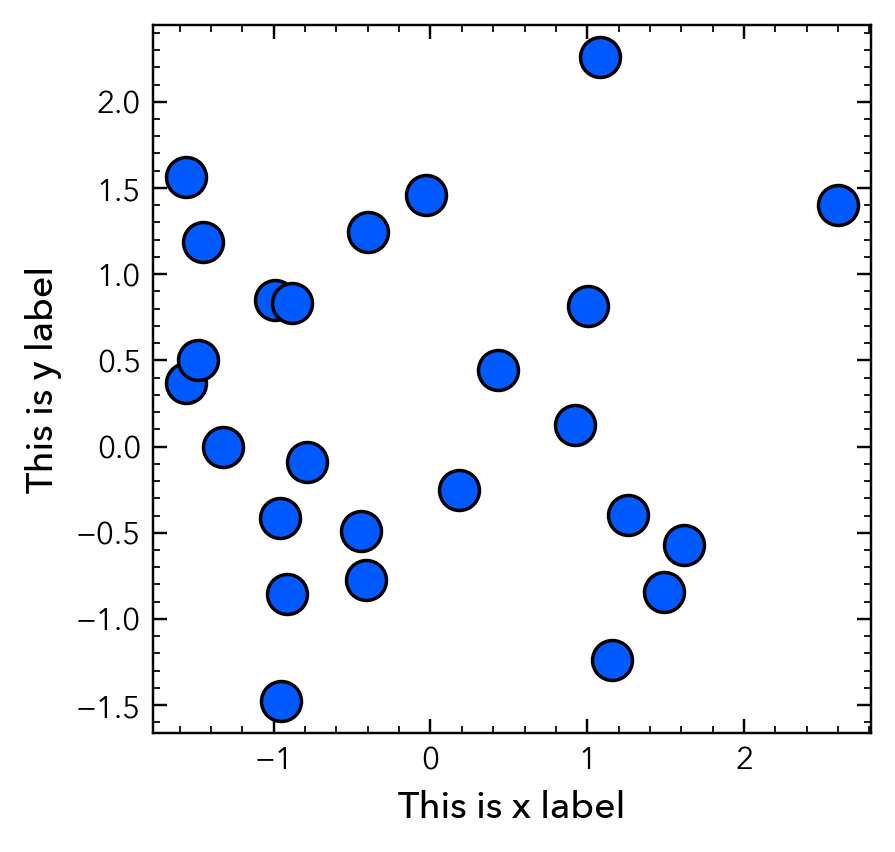
\includegraphics[width=1.0\linewidth]{./obipy-resources/fiducial.png}
\end{center}
\section{目盛り}
\label{sec:org2344501}
\subsection{目盛りの数字}
\label{sec:orgfb6ce28}
目盛りの軸ラベルのサイズを変更し、縦軸の目盛りを指定する。
\begin{minted}[frame=lines,framesep=2mm,linenos=true,breaklines]{ipython}
ax = plot_fiducial()
ax.tick_params(labelsize='xx-small')    # both axes
ax.tick_params(axis='y', labelsize=20)
_ = ax.set_yticks([-0.5, 1.5, 2.0])
\end{minted}

\begin{center}
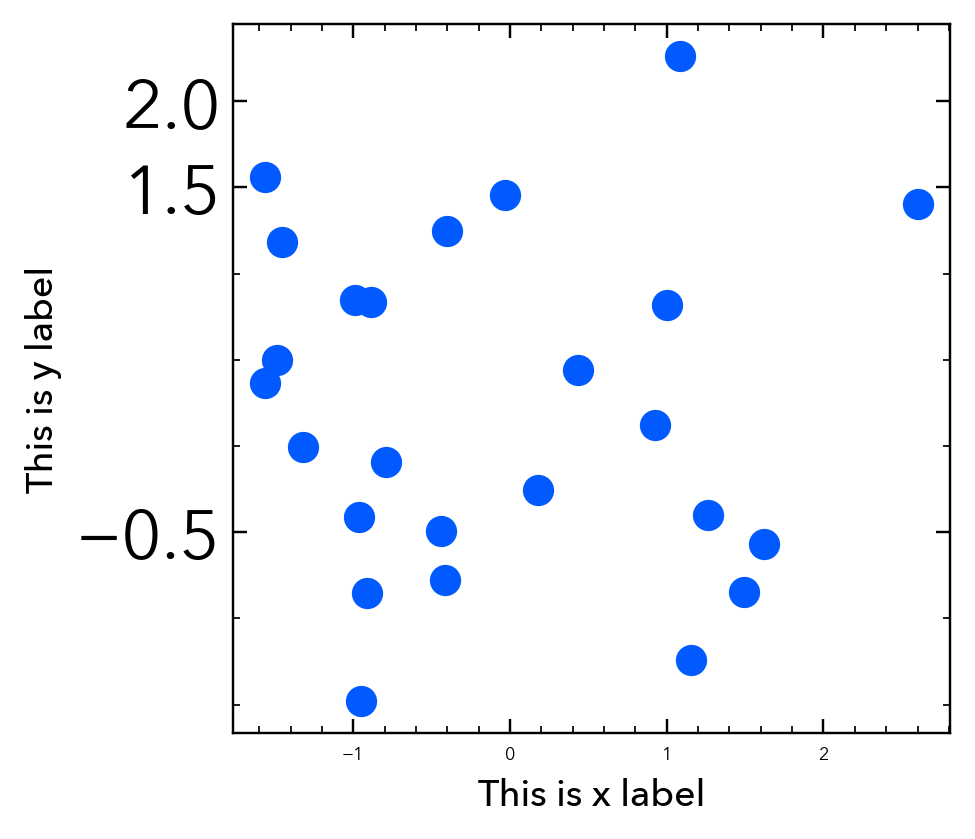
\includegraphics[width=1.0\linewidth]{./obipy-resources/params_ticks.png}
\end{center}
\section{矢印}
\label{sec:org6b68ac0}
\subsection{arrow}
\label{sec:org1009cfc}
データ座標を使って矢印を描く。
\begin{minted}[frame=lines,framesep=2mm,linenos=true,breaklines]{ipython}
ax = plot_fiducial()
_ = ax.arrow(
    x=-1.0,
    y=-0.5,
    dx=1.0,
    dy=1.4,
    width=0.05,
    head_length=0.3,
    length_includes_head=True,
    fc='red',
)
\end{minted}

\begin{center}
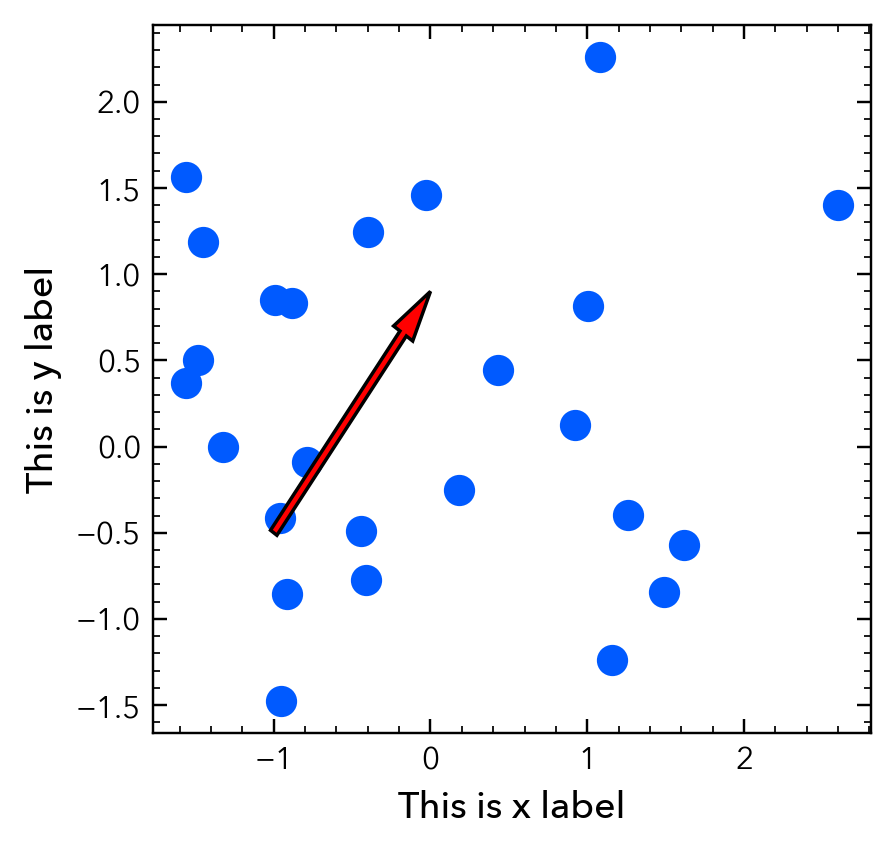
\includegraphics[width=1.0\linewidth]{./obipy-resources/params_arrow.png}
\end{center}
\section{大量の線}
\label{sec:org4dddadb}
一斉に同じ種類の線をプロットするには \texttt{mcoll.LineCollection} を使って、返り値を \texttt{ax.add\_collection()} で加えると良い。
\begin{minted}[frame=lines,framesep=2mm,linenos=true,breaklines]{ipython}
import matplotlib.collections as mcoll
from sugayutils import colors

ax = plot_fiducial()
segments = (
    ((-1.0, 0.0), (1.0, 0.0)),
    ((-1.0, 0.5), (1.0, 0.5)),
    ((-1.0, 1.0), (1.0, 1.0)),
    ((-1.0, 1.5), (1.0, 1.5)),
    ((-1.0, 2.0), (1.0, 2.0)),
    ((0.0, -1.0), (0.0, 1.0)),
)
linecollection = mcoll.LineCollection(segments, colors=colors.green, lw=0.5, ls='--')
_ = ax.add_collection(linecollection)
\end{minted}

\begin{center}
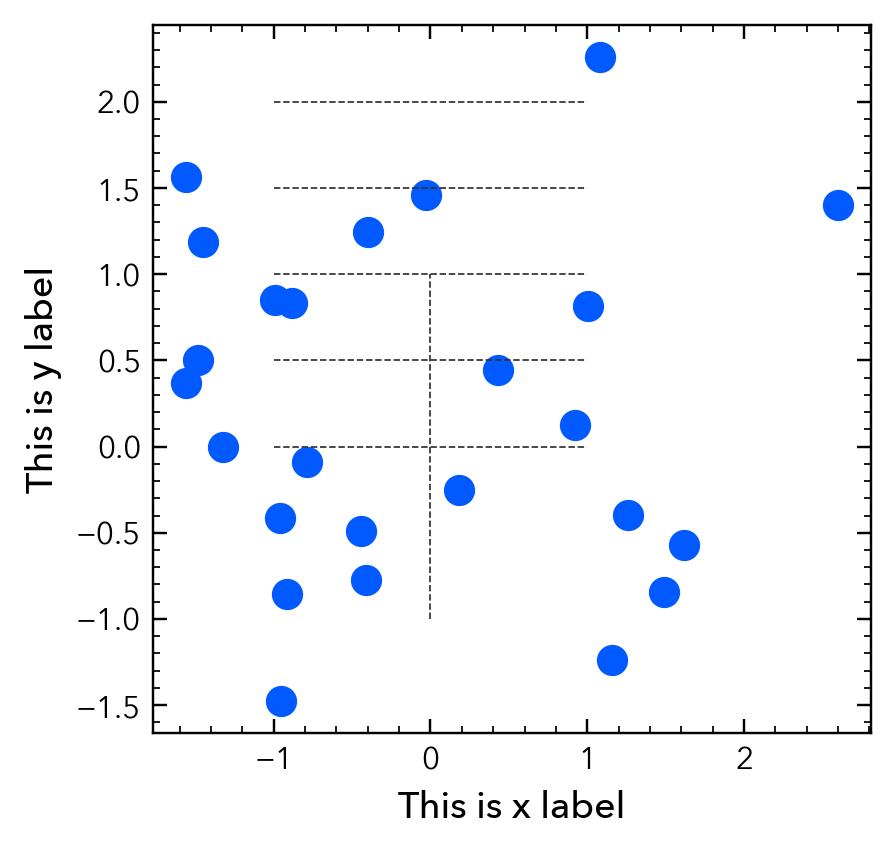
\includegraphics[width=1.0\linewidth]{./obipy-resources/params_lines.png}
\end{center}
\end{document}
